\section{Implementierung}
\label{implementierung}
\subsection{Abhängigkeiten und Exklusitiväten}
Im Rahmen der Abhängigkeiten und Exklusivitäten von Erweiterungen zueinander gibt es mehrere Probleme, die gelöst werden müssen. Zum einen kann es schnell passieren, eine unmögliche Kombination von Bedingungen zu stellen. Außerdem muss nach der Auswahl einer Kombination von Erweiterungen geprüft werden, ob diese Kombination zulässig ist.

\subsubsection{Überprüfung der Umsetzbarkeit}


Ein triviales Beispiel für unmögliche Kombinationen von Bedingungen wäre ein Paar von Abhängigkeiten $A$ und $B$, wobei $A$ und $B$ exklusiv zueinander sind und gleichzeitig $A$ von $B$ abhängt. Es können in diesem Beispiel niemals beide Anforderungen gleichzeitig erfüllt werden.

Natürlich lassen sich aber auch kompliziertere Beispiele erzeugen. In Abbildung \ref{fig:impl:dependency_conflict_examples} werden zwei solche Konstellation dargestellt. Bei der einen hängt $A$ von $B$ und $B$ von $C$ ab, aber $A$ ist zu $C$ exklusiv. Diese Kombination von Anforderungen lässt sich ebensowenig wie das erste Beispiel gleichzeitig erfüllen, aber das Problem ist hier nicht sofort offensichtlich. Man muss hierfür erkennen, dass Abhängigkeiten transitiv sind. Ist also die Erweiterung $A$ von $B$ und $B$ von $C$ abhängig, so ist auch indirekt $A$ von $C$ abhängig.

  \begin{figure}
		\centering
		\begin{subfigure}[a]{0.4\linewidth}
			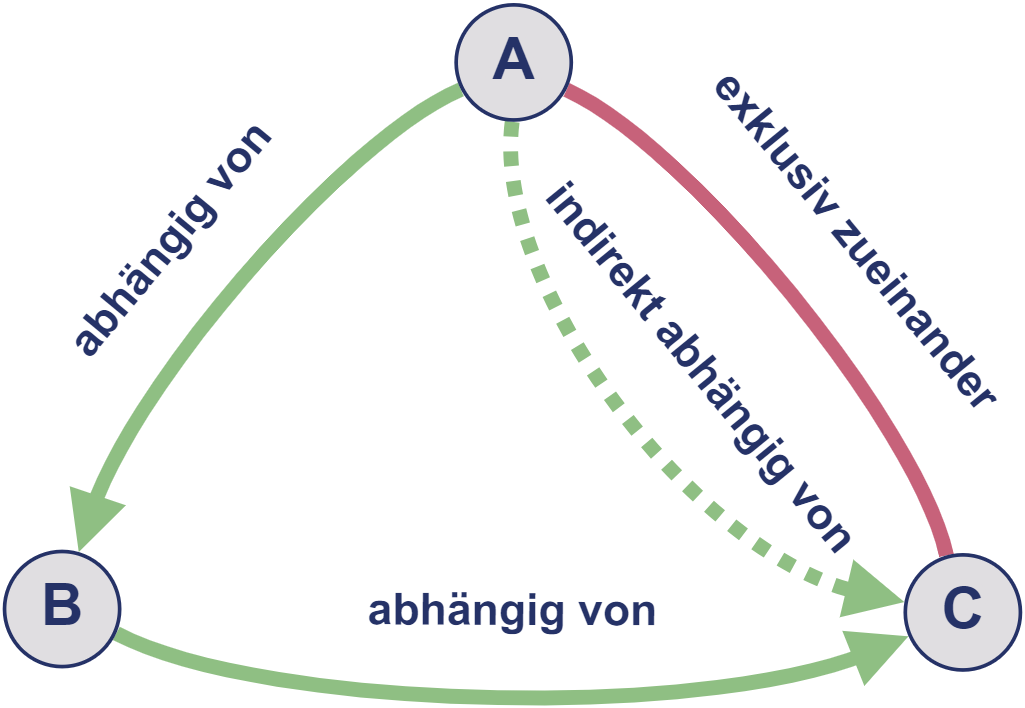
\includegraphics[width=\linewidth]{dependency_example_1.png}
      		\caption{Eine Möglichkeit, wie ein Widerspruch zwischen indirekter Abhängigkeit und Exklusivität entstehen kann.}
		\end{subfigure}
		\begin{subfigure}[a]{0.4\linewidth}
			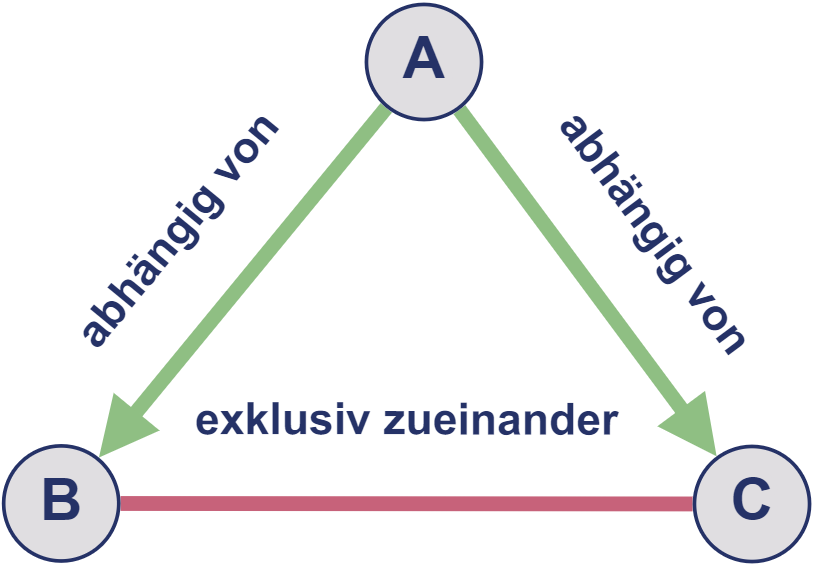
\includegraphics[width=\linewidth]{dependency_example_2.png}
      		\caption{Hier entsteht ein Widerspruch dadurch, dass eine Erweiterung zwei Abhängigkeiten hat, die zueinander exklusiv sind.}
		\end{subfigure}
		\caption{Zwei Graphen zur Veranschaulichung von Konfliktmöglichkeiten zwischen Abhängigkeiten und Exklusivitäten.}
		\label{fig:impl:dependency_conflict_examples}
  \end{figure}

Der zweite in Abbildung \ref{fig:impl:dependency_conflict_examples} dargestellte Konflikt beruht im Gegensatz zu den bisherigen Beispielen nicht darauf, dass eine Erweiterung zugleich (indirekt) abhängig und exklusiv zu einer anderen Erweiterung ist. Hier wird eine weitere Kategorie von Problemen dargestellt: sind zwei (indirekte) Abhängigkeiten einer Erweiterung zueinander exklusiv, so können nicht beide dieser Abhängigkeiten erfüllt werden. Auch solche Konfigurationen sind also unzulässig.

Aus diesen fachlichen Überlegungen heraus ergibt sich eine erste Lösung. Für jede Erweiterung $E$ sind zunächst alle direkten sowie indirekten Abhängigkeiten zu bestimmen. Für alle diese Abhängigkeiten ist dann zu prüfen, dass zum einen die Abhängigkeit $A$ nicht zu $E$ exklusiv ist, aber auch dass $A$ zu keiner weiteren (indirekten) Abhängigkeit $A'$ von $E$ exklusiv ist.

Bei näherer Betrachtung dieser Lösung lässt sich jedoch einiges an Ineffizienz feststellen. Zum einen werden für jede Erweiterung erneut die transitiven Abhängigkeiten berechnet. Aufgrund eben dieser Transitivität sind jedoch die Berechnungen für alle Erweitungen, die Abhängigkeit einer anderen Erweiterung sind, redundant. Im schlimmsten Fall (nämlich, wenn eine Erweiterung von insgesamt $n$ Erweiterungen von allen anderen Erweiterungen (indirekt) abhängt) ist also genau eine der durchgeführten Berechnungen wirklich notwendig und $n - 1$ Berechnungen werden unnötigerweise durchgefüht. Aus ähnlichem Grund ist auch die Überprüfung der Exklusitivät zweier paarweise unabhängiger (indirekter) Abhängigkeiten häufig überflüssig.

Die Lösung dieser Probleme ergibt sich aus einer theoretischeren Betrachtung des Problems. Wie bereits aus der Verwendung des Begriffs der Transitivität hervorgeht, lassen sich Abhängigkeit und Exklusitivät als mathematische Relationen über der Menge aller Erweiterungen auffassen. Hierbei ist besonders hervorzuheben, dass die Exklusivität symmetrisch ist (ist $A$ zu $B$ exklusiv, so ist auch $B$ zu $A$ exklusiv) während Abhängigkeit nicht symmetrisch ist (im Gegenteil: bei der anfänglichen Analyse von möglichen Bibliotheken, Frameworks etc. ergab sich, dass Abhängigkeit nie symmetrisch zu sein scheint). Allerdings ist Exklusivität a priori nicht transitiv (auch, wenn $A$ zu $B$ und $B$ zu $C$ exklusiv ist, können $A$ und $C$ zusammen verwendet werden), während Abhängigkeit sehr wohl transitiv ist (wie bereits erläutert).

Vor diesem Hintergrund lässt sich erkennen, dass die Bestimmung der (indirekten) Abhängigkeiten der Bestimmung der Transitiven Hülle gleichkommt. Diese kann mittels des Floyd-Warshall-Algorithmus (in der Warshall-Variante) berechnet werden \cite{warshal1_algorithm}. Hierfür muss zunächst ein gerichteter Graph erzeugt werden, in den alle deklarierten Abhängigkeiten als Kante eingefügt werden. Von diesem Graphen wird dann die transitive Hülle bestimmt, in der zwei Knoten $A$ und $B$ genau dann durch eine (von $A$ nach $B$ gerichtete) Kante verbunden sind, wenn die Erweiterung $A$ von $B$ abhängt.

Auch die Relation der Exklusivität lässt sich in einen Graphen überführen. In diesem Graphen gibt es ebenfalls pro Erweiterung einen Knoten und jede Exklusivität wird als Kante dargestellt. Aufgrund der Symmetrie der Exklusivität kann dieser Graph aber ungerichtet sein.

Das Problem der Überprüfung der Restriktionen reduziert sich nun darauf, sicherzustellen, dass es zwischen zwei Knoten (also zwischen zwei Erweiterungen) in maximal einem der beiden Graphen eine Kante gibt, wobei die Richtung keine Rolle spielt (denn wenn die Knoten exklusiv zueinander sind, darf es zwischen beiden keine Abhängigkeit geben -- egal, in welche Richtung).

Anders formuliert, darf es im Graphen der Exklusivitäten keine Kante $\{A, B\}$ geben, für die in der transitiven Hülle der Abhängigkeiten die Kante $(A, B)$ oder die Kante $(B, A)$ existiert. Aufgrund dessen, dass die transitive Hülle gerichtet ist, gibt es darin doppelt so viele Kanten wie in dem Graphen der Exklusivitäten. Außerdem liegt sie als Adjazenzmatrix vor, während die Exklusivitäten als Kantenliste vorliegen. Somit kann bei $m$ Exklusivitäten in $\mathcal{O}(m)$ über die Exklusivitäten iterieren und jeweils in $\mathcal{O}(1)$ die Existenz einer (transitiven) Abhängigkeit prüfen. Die Umkehrung, also die Iteration über Abhängigkeiten und dann die Prüfung der Existenz einer Exklusivität, würde bei $n$ Erweiterungen einen Aufwand von $\mathcal{O}(n^2)$ verursachen. Wenn man vorher die Kantenliste der Exklusivitäten in $\mathcal{O}(n^2)$ in eine Adjazenzmatrix überführt, ist die anschließende Existenzprüfung auch wieder in $\mathcal{O}(1)$ möglich, aber insgesamt

Der Algorithmus von Floyd-Warshall sorgt dafür, dass diese Überprüfung eine asymptotische Laufzeit von $\mathcal{O}(n^3)$ hat. Da die oben beschriebenen Probleme in beliebiger Tiefe von Abhängigkeiten auftreten können, ist jedoch die Bestimmung der transitiven Hülle nicht vermeidbar. Allerdings ist damit zu rechnen, dass die Anzahl aller Erweiterungen stets kleiner als $100$ sein wird (andernfalls würde die Benutzbarkeit des Programms möglicherweise stark eingeschränkt). Daher ist diese Laufzeit in diesem Fall als unbedenklich einzustufen.